\newpage
\section{Đề thi Giải tích}

\begin{tcolorbox}[title=\textbf{Bài toán B.1 + A.1.},breakable]
    Cho $(a_n)$ là dãy số thực được xác định bởi các điều kiện $$a_1 = 1,\quad a_{n+1} = a_n + \dfrac{(-1)^n}{n!} \,\forall n \geq 1.$$
    \begin{enumerate}
        \item[(a)] {Tìm tất cả các số nguyên dương $n$ sao cho $a_n \geq \dfrac{1}{2}$.}
        \item[(b)] {Chứng minh rằng dãy số $(a_n)$ hội tụ.} 
        \item[(c)] Giới hạn của dãy số $(a_n)$ là một số hữu tỷ hay vô tỷ? Vì sao? 
    \end{enumerate}
\end{tcolorbox}

\textbf{Lời giải. }

\begin{enumerate}
    \item[(a)] {Bằng tính toán, ta có $a_1 = 1,\,a_2 = 0,\,a_3 = \dfrac{1}{2},\,a_4 = \dfrac{1}{3},\,a_5 = \dfrac{3}{8}$. Ta sẽ chứng minh rằng $a_n < \dfrac{1}{2}$ với mọi $n > 3$. 
    
    Thật vậy, mệnh đề cần chứng minh đúng với $n = 4$ và $n = 5$. Giả sử mệnh đề đúng đến $n = 2k$ và $n = 2k + 1$ (trong đó $k \in \mathbb{Z^+}$), tức đã có $a_{2k} < \dfrac{1}{2}$ và $a_{2k+1} < \dfrac{1}{2}$. Ta có $$a_{2k + 2} = a_{2k+1} - \dfrac{1}{(2k + 1)!} < \dfrac{1}{2}$$ và $$a_{2k+3} = a_{2k+2} + \dfrac{1}{(2k+2)!} = a_{2k+1} - \dfrac{1}{(2k+1)!}+ \dfrac{1}{(2k+2)!} = a_{2k+1} - \dfrac{2k}{(2k+2)!} < \dfrac{1}{2}.$$
    
    Như vậy theo nguyên lý quy nạp toán học, $a_n < \dfrac{1}{2}$ với mọi $n > 3$. Do đó tất cả các số nguyên dương $n$ thỏa mãn $a_n \geq \dfrac{1}{2}$ là 1 và 3.} 
    \item[(b)] {Với mọi $n\geq 2$ ta có $$a_n = a_{n-1} + \dfrac{(-1)^{n-1}}{(n-1)!} = a_{n-2} + \dfrac{(-1)^{n-1}}{(n-1)!} + \dfrac{(-1)^{n-2}}{(n-2)!} = \cdots = a_1 + \sum\limits_{i = 1}^{n-1}\dfrac{(-1)^{i}}{i!} = 1 + \sum\limits_{i = 1}^{n-1}\dfrac{(-1)^{i}}{i!}.$$
    
    Xét hàm số $f(x) = {\rm e}^{-x}$. Ta thấy $$f^{(n)}(x) = \begin{cases}
        -{\rm e}^{-x},\quad &\text{nếu $n$ lẻ} \\
        {\rm e}^{-x},\quad &\text{nếu $n$ chẵn}  
    \end{cases},$$ trong đó $f^{(n)}(x)$ là đạo hàm cấp $n$ của hàm số $f$. Theo khai triển Maclaurin, ta có $$f(x) = 1 + \dfrac{-1}{1!}x + \dfrac{1}{2!}x^2 + \cdots + \dfrac{(-1)^{n-1}}{(n-1)^n}x^{n-1} + \dfrac{(-1)^n \cdot {\rm e}^{-c}}{n!}x^n,$$
    trong đó $c$ là số thực nào đó nằm giữa 0 và $x$.
    
    Từ đây suy ra $$\dfrac{1}{{\rm e}} = f(1)  = 1 + \dfrac{-1}{1!} + \dfrac{1}{2!} + \cdots + \dfrac{(-1)^{n-1}}{(n-1)^n} + \dfrac{(-1)^n \cdot {\rm e}^{-c}}{n!}= a_n + \dfrac{(-1)^n \cdot {\rm e}^{-c}}{n!},$$ với $c$ là số thực nào đó thỏa mãn $0 < c < 1$, với mọi $n \geq 2$.
    
    Do đó với mọi $n \geq 2$ thì $$\left|a_n - \dfrac{1}{{\rm e}}\right| = \dfrac{{\rm e}^{-c}}{n!}, $$ với $c$ là số thực nào đó thỏa mãn $0 < c < 1$.
    
    Trong đẳng thức trên, cho $n \to +\infty$, để ý rằng $\dfrac{{\rm e}^{-c}}{n!} \to 0$, ta thu được $\lim\limits_{n\to +\infty}a_n = \dfrac{1}{{\rm e}}$. Như vậy dãy số $(a_n)$ hội tụ.} 
    \item[(c)] {Theo câu (b), ta có $\lim\limits_{n\to +\infty}a_n = \dfrac{1}{{\rm e}}$ là một số vô tỷ.} 
\end{enumerate}

\textbf{Nhận xét. }Đây là một bài toán giới hạn dãy số liên quan giới hạn của chuỗi số. Câu (a) là một câu cơ bản, đòi hỏi việc tính toán một số giá trị đầu của dãy số và kỹ năng chứng minh quy nạp. Câu (b) có thể tách dãy số đã cho làm hai dãy con chẵn và lẻ, từ đó sử dụng định nghĩa để chứng minh; cách giải đề xuất ở đây có phần gọn hơn, nhưng đòi hỏi phải nhận xét được dãy số đã cho liên quan đến khai triển Maclaurin của hàm $f(x) = {\rm e}^{-x}$. Tuy nhiên cách giải được đề xuất ở đây lại hiệu quả trong việc chỉ ra chính xác giới hạn của dãy $(a_n)$ là $\dfrac{1}{{\rm e}}$.

\begin{tcolorbox}[title=\textbf{Bài toán B.2 + A.2.},breakable]
    Cho $f:\,\mathbb{R} \to \mathbb{R}$ là hàm số được xác định bởi công thức $$f(x) = \begin{cases}
        ax^2+b,\quad &\text{nếu $x \leq 0$} \\
        {\rm e}^x + cx,\quad &\text{nếu $x > 0$}  
    \end{cases},$$trong đó $a,\,b,\,c$ là các tham số thực.
    \begin{enumerate}
        \item[(a)] {Xác định $a,\,b,\,c$ sao cho hàm $f$ liên tục trên $\mathbb{R}$.}
        \item[(b)] {Xác định $a,\,b,\,c$ sao cho hàm $f$ khả vi trên $\mathbb{R}$.} 
        \item[(c)] {Xác định $a,\,b,\,c$ sao cho hàm $f$ khả vi cấp hai trên $\mathbb{R}$.} 
    \end{enumerate}
\end{tcolorbox}

\textbf{Lời giải. }

\begin{enumerate}
    \item[(a)] {Với $x \leq 0$ thì $f(x) = ax^2 + b$, còn với $x > 0$ thì $f(x) = {\rm e}^x + cx$ nên $f$ liên tục tại mọi điểm khác 0. Do đó để $f$ liên tục trên $\mathbb{R}$ thì $f$ cần phải liên tục tại $0$.
        
    Ta có $$\lim\limits_{x \to 0^-}f(x) = \lim\limits_{x \to 0^-} (ax^2 + b) = b,\quad \lim\limits_{x \to 0^+}f(x) = \lim\limits_{x \to 0^+}({\rm e}^x + cx) = 1 = f(0).$$ 
    
    Để $f$ liên tục tại $0$ thì $\lim\limits_{x \to 0^-}f(x) = \lim\limits_{x \to 0^+}f(x) = f(0)$ hay $b = 1$. Như vậy khi $b = 1$ và $a,\,c$ tùy ý thì $f$ liên tục trên $\mathbb{R}$.}
    \item[(b)] {Nhận xét rằng $f$ khả vi tại mọi điểm khác 0. Do đó để $f$ khả vi trên $\mathbb{R}$ thì $f$ cần phải khả vi tại 0. Điều này tương đương với $$\begin{cases}
        \text{$f$ liên tục tại 0} \\
        \text{$\lim\limits_{x \to 0}\dfrac{f(x) - f(0)}{x}$ tồn tại}
    \end{cases}.$$
    
    Theo câu $(a)$, để $f$ liên tục tại 0 thì $b = 1$. 
    
    Ta có $$\lim\limits_{x \to 0^-}\dfrac{f(x) - f(0)}{x} = \lim\limits_{x \to 0^-}\dfrac{ax^2 + b - b}{x} = \lim\limits_{x \to 0^-}ax = 0$$ và $$\lim\limits_{x \to 0^+}\dfrac{f(x) - f(0)}{x} = \lim\limits_{x \to 0^+}\dfrac{{\rm e}^x + cx - 1}{x} = c + 1,$$ để ý rằng $\lim\limits_{x \to 0^+} \dfrac{{\rm e}^x-1}{x} = \lim\limits_{x \to 0^+} \dfrac{{\rm e}^x}{1} = 1$ theo quy tắc l'Hospital.
    
    Do đó để $\lim\limits_{x \to 0}\dfrac{f(x) - f(0)}{x}$ tồn tại thì $\lim\limits_{x \to 0^-}\dfrac{f(x) - f(0)}{x} = \lim\limits_{x \to 0^+}\dfrac{f(x) - f(0)}{x}$ hay $c = -1$. Như vậy, khi $b = 1,\,c = -1$ và $a$ tùy ý thì $f$ khả vi trên $\mathbb{R}$.}
    \item[(c)] {Để $f$ khả vi cấp hai trên $\mathbb{R}$ thì trước hết $f$ phải khả vi cấp một trên $\mathbb{R}$. Theo câu (b), để $f$ khả vi cấp một trên $\mathbb{R}$ thì $b = 1,\,c = -1$ và khi đó $$f'(x) = \begin{cases}
        2ax,\quad &\text{nếu $x \leq 0$} \\
        {\rm e}^x - 1,\quad &\text{nếu $x > 0$} \\
        \lim\limits_{x \to 0}\dfrac{f(x) - f(0)}{x} = 0,\quad &\text{nếu $x = 0$} 
    \end{cases}$$
        
    Nhận xét rằng $f$ khả vi cấp hai tại mọi điểm khác 0. Do đó để $f$ khả vi cấp hai trên $\mathbb{R}$ thì $f$ cần phải khả vi cấp hai tại 0. Điều này tương đương với $$\begin{cases}
        \text{$f'$ liên tục tại 0} \\
        \text{$\lim\limits_{x \to 0}\dfrac{f'(x) - f'(0)}{x}$ tồn tại}
    \end{cases}.$$
    
    Ta có $$\lim\limits_{x \to 0^-}f'(x) = \lim\limits_{x \to 0^-} (2ax) = 0,\quad \lim\limits_{x \to 0^+}f'(x) = \lim\limits_{x \to 0^+} ({\rm e}^x -1) = 0 = f'(0).$$
    
    Vì $\lim\limits_{x \to 0^-}f'(x) = \lim\limits_{x \to 0^+}f'(x) = f'(0)$ nên $f'$ liên tục tại 0.
    
    Ta lại có $$\lim\limits_{x \to 0^-}\dfrac{f'(x)-f'(0)}{x} = \lim\limits_{x \to 0^-}\dfrac{2ax}{x} = 2a$$ và $$\lim\limits_{x \to 0^+}\dfrac{f'(x)-f'(0)}{x} = \lim\limits_{x \to 0^+}\dfrac{{\rm e}^x - 1}{x} = 1.$$
    
    Do đó để $\lim\limits_{x \to 0}\dfrac{f'(x) - f'(0)}{x}$ tồn tại thì $\lim\limits_{x \to 0^-}\dfrac{f'(x) - f'(0)}{x} = \lim\limits_{x \to 0^+}\dfrac{f'(x) - f'(0)}{x}$ hay $a = \dfrac{1}{2}$. Như vậy, khi $a = \dfrac{1}{2},\,b = 1,\,c = -1$ thì $f$ khả vi cấp hai trên $\mathbb{R}$.}
\end{enumerate}

\textbf{Nhận xét. }Đây là một bài toán cơ bản về tính liên tục và khả vi của hàm số. Để giải quyết bài toán này đòi hỏi phải nắm vững tính chất về tính liên tục và tính khả vi.

Để hàm số $f$ liên tục tại điểm $x = x_0$ thì $f$ phải thỏa mãn đồng thời ba điều kiện 
\begin{enumerate}
    \item[(i)] {$f$ xác định tại $x_0$;}
    \item[(ii)] {$\lim\limits_{x\to x_0}f(x)$ tồn tại;}
    \item[(iii)] {$\lim\limits_{x\to x_0}f(x) = f(x_0)$.}
\end{enumerate}

Còn để hàm số $f$ khả vi tại điểm $x = x_0$ thì $f$ phải thỏa mãn đồng thời hai điều kiện 
\begin{enumerate}
    \item[(i)] {$f$ liên tục tại điểm $x = x_0$;}
    \item[(ii)] {$\lim\limits_{x\to x_0}\dfrac{f(x) - f(x_0)}{x - x_0}$ tồn tại.}
\end{enumerate}
khi đó $\lim\limits_{x\to x_0}\dfrac{f(x) - f(x_0)}{x - x_0}$ là đạo hàm của hàm số $f$ tại điểm $x = x_0$ hay $f'(x_0)$.

\begin{tcolorbox}[title=\textbf{Bài toán B.3 + A.3.},breakable]
    Hình vẽ bên thể hiện một phần đường thẳng $(d)$ có phương trình $$y = 2x - 1$$ và một phần parabol $(P)$ có phương trình $$y = 3x^2$$ trong mặt phẳng tọa độ $Oxy$.
    \begin{center}
        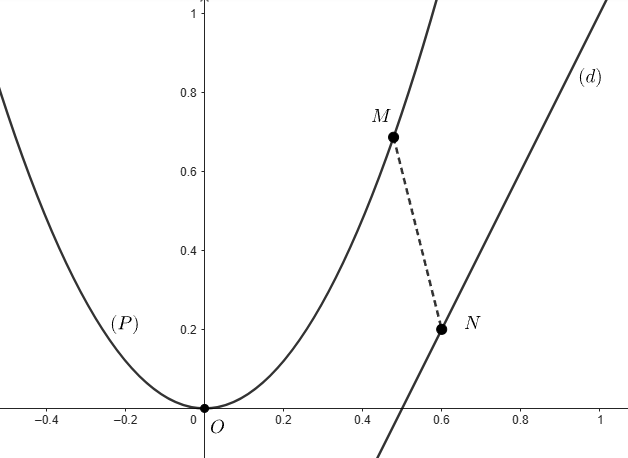
\includegraphics[width=0.5\textwidth]{Figures/04.png}
    \end{center}
    \begin{enumerate}
        \item[(a)] {Đường thẳng $(d)$ và parabol $(P)$ có cắt nhau không? Vì sao?}
        \item[(b)] {Cho các điểm $M \in (P)$ và $N\in (d)$. Tìm giá trị nhỏ nhất của khoảng cách $MN$.} 
    \end{enumerate}
\end{tcolorbox}

\textbf{Lời giải. }



\begin{tcolorbox}[title=\textbf{Bài toán B.4.},breakable]
    Cho $f:\,[0;\,1] \to \mathbb{R}$ là một hàm số liên tục trên $[0;\,1]$ và khả vi trong $(0;\,1)$.

    \begin{enumerate}
        \item[(a)] {Chứng minh rằng nếu $f(1) = 0$ thì tồn tại một số thực $x_0 \in (0;\,1)$ sao cho $$|f(x_0)| \leq 2024|f'(x_0)|.$$}
        \item[(b)] {Chứng minh rằng nếu $f(1) = 0$ và $$|f(x)| \geq 2024|f'(x)|\text{ với mọi }x \in (0;\,1)$$ thì $f$ là hàm hằng.}
        \item[(c)] {Khẳng định trong ý (b) có còn đúng không nếu ta không giả thiết $f(1) = 0$ (nếu câu trả lời là "có", hãy chứng minh; nếu câu trả lời là "không", hãy chỉ ra ví dụ về một hàm số $f$)?}  
    \end{enumerate}
\end{tcolorbox}

\textbf{Lời giải. }

\begin{tcolorbox}[title=\textbf{Bài toán B.5.},breakable]
    Cho $D$ là một phần của mặt phẳng tọa độ $Oxy$ gồm những điểm có tọa độ $(x;\,y)$ mà $$0 \leq x \leq \dfrac{\pi}{2}$$ và $$0 \leq y \leq \dfrac{(\cos x)^4}{(\sin x)^4 + (\cos x)^4}\text{ với }0 \leq x \leq \dfrac{\pi}{2}.$$
    \begin{center}
        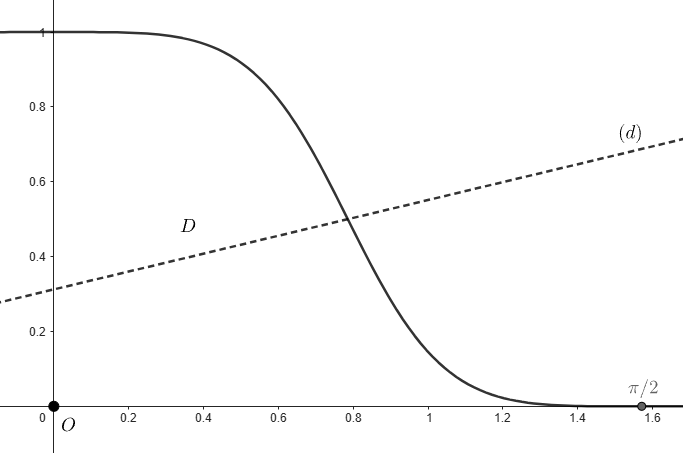
\includegraphics[width=0.5\textwidth]{Figures/05.png}
    \end{center}
    \begin{enumerate}
        \item[(a)] {Tính diện tích của $D$.}
        \item[(b)] {Cho $(d)$ là một đường thẳng đi qua hai điểm $\left(\dfrac{\pi}{4};\,\dfrac{1}{2}\right)$ và $(0;\,a)$ với $0 < a < 1$. Người ta muốn cắt $D$ dọc theo $(d)$ để thu được hai phần rời nhau có cùng diện tích (hình vẽ trong bài thể hiện một cách cắt dọc theo đường nét đứt). Coi việc cắt không làm ảnh hưởng đến diện tích của $D$. Xác định giá trị của $a$ tương ứng với một cách cắt thỏa mãn yêu cầu.} 
    \end{enumerate}
\end{tcolorbox}

\textbf{Lời giải. }